\documentclass{beamer}
\usetheme{metropolis}
\usepackage{graphicx}
\usepackage{amsmath}
\title{Digital Signal Processing: COSC390}
\author{Jordan Hanson}
\institute{Whittier College Department of Physics and Astronomy}

\begin{document}
\maketitle

\begin{frame}{Course Introduction}
\begin{enumerate}
\item\textit{ \textbf{\alert{What is digital signal processing?}}}
\item \textit{COSC330: Computer Logic and Digital Circuit Design}
\item Read the syllabus for a roadmap
\item \textit{This course can be fast.}
\item \textbf{Data science project and presentation}
\item Textbook: \url{http://dspguide.com}
\item Download and install octave: \url{https://www.gnu.org/software/octave}
\end{enumerate}
\end{frame}

\begin{frame}{Lecture format, with modifications}
\begin{itemize}
\item Theory and examples
\item Programming with Octave
\item Application
\item Study hall
\begin{enumerate}
\item Homework help
\item Project and presentation development
\item Special topics lectures
\end{enumerate}
\end{itemize}
\end{frame}

\begin{frame}{Unit 1.1 Outline}
\begin{enumerate}
\item Complex numbers 1: Arithmetic and some calculus (continuous and discete)
\item Complex numbers 2: The Fourier series and Fourier transform (continuous and discrete)
\item \textit{Time-permitting}: The Laplace transform (continuous and discrete)
\end{enumerate}
\end{frame}

\section{Complex numbers 1}

\begin{frame}{Complex numbers 1: Definition of a complex number}
A \alert{complex number} is an expression for which one term is proportional to $j = \sqrt{-1}$:
\begin{equation}
z = x + jy
\end{equation}
To call the \textit{complex unit} $j$ is the convention in electrical engineering, and in physics it is often called $i$. \\ \vspace{0.5cm}
Example of complex numbers: $(3+4j)$, $(x_1 + x_2 j)$.  Each number has a \textit{real} part and an \textit{imaginary} part.
\end{frame}

\begin{frame}{Complex numbers 1: Definition of a complex number}
Operations to learn:
\begin{enumerate}
\item Addition
\item Subtraction
\item Real part $\operatorname{Re}$ and $\operatorname{Im}$
\item Multiplication
\item Division
\item Conjugation
\item Magnitude/Norm
\end{enumerate}
\end{frame}

\begin{frame}{Complex numbers 1: Operations}
Addition follows the pattern of two-dimensional vectors:
\begin{align}
z_1 &= 3+4j \\
z_2 &= -2+5j \\
z_1 + z_2 &= 1+9j
\end{align} \\
Subtraction follows the pattern of two-dimensional vectors:
\begin{align}
z_1 &= 3+4j \\
z_2 &= -2+5j \\
z_1 - z_2 &= 5-1j
\end{align}
\end{frame}

\begin{frame}{Complex numbers 1: Operations}
\begin{figure}
\centering
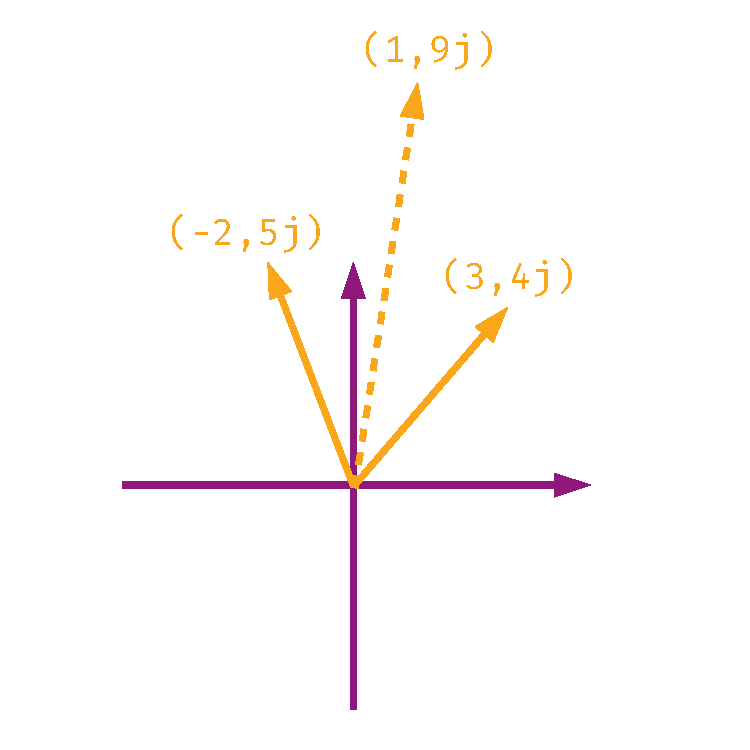
\includegraphics[width=0.45\textwidth]{figures/complexNumbers1.pdf}
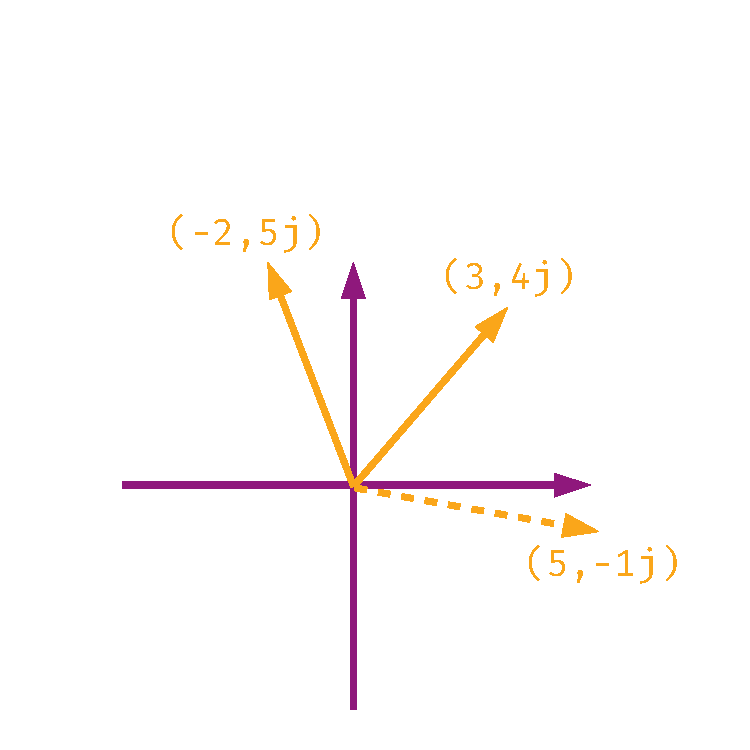
\includegraphics[width=0.45\textwidth]{figures/complexNumbers2.pdf}
\caption{\label{fig:complex1} Complex addition and subtraction follows the pattern of two-dimensional vectors.}
\end{figure}
\end{frame}

\begin{frame}{Complex numbers 1: Operations}
We also have the $\operatorname{Re}$ and $\operatorname{Im}$ operations:
\begin{align}
z_1 &= 3+4j \\
\operatorname{Re}\lbrace z_1 \rbrace &= 3 \\
\operatorname{Im}\lbrace z_2 \rbrace &= 4
\end{align}
These are known as taking the \textit{real}-part and the \textit{imaginary}-part.  The original complex number can be recovered by adding real and imaginary parts together:
\begin{equation}
z_1 = \operatorname{Re}\lbrace z_1 \rbrace + j \operatorname{Im}\lbrace z_1 \rbrace
\end{equation} \\
When we add/subtract complex numbers, we combine the real parts and imaginary parts separately.
\end{frame}

\begin{frame}{Complex numbers 1: Operations}
\textit{Add or subtract, then simplify:}
\begin{enumerate}
\item $z_1 = 7+7j$, $z_2 = -6+3j$.  $z_1+z_2 = $
\item $z_1 = 2+2j$, $z_2 = 3-3j$.  $z_1-z_2 = $
\item $z_1 = 2x+7j$, $z_2 = 2+4xj$.  $z_1+z_2 = $
\end{enumerate}
Let $x=-1$ and $y=1$.  \textit{Evaluate the following expressions:}
\begin{enumerate}
\item $z_1 = x+yj$, $z_2 = y+xj$.  $z_1+z_2 = $
\item $z_1 = x^2+y^2j$, $z_2 = 2y^2+x^2j$.  $z_1-z_2 = $
\end{enumerate}
\end{frame}

\begin{frame}{Complex numbers 2: Operations}
\textit{Multiplication: Recall that $j^2 = -1$.}
\begin{align}
z_1 &= x_1+jy_1 \\
z_2 &= x_2 + j y_2 \\
z_1 \times z_2 &= x_1 x_2 - y_1 y_2 + j (x_1 y_2 + x_2 y_1)
\end{align}
The cross-terms are straightforward, but remember the minus sign when multiplying the imaginary parts.
\end{frame}

\section{Complex numbers 2}

\section{Conclusion}

\begin{frame}{Conclusion}
Text
\end{frame}

\end{document}
